% DPF 09 talk on strangeness in nucleon

\documentclass[10pt]{beamer}
\usepackage{amsmath}
\usepackage{mathtools}
\usefonttheme{professionalfonts} % using non standard fonts for beamer
\usefonttheme{serif} % default family is serif

%\documentclass[12pt]{beamerthemeSam.sty}
\usepackage{epsf}
%\usepackage{pstricks}
%\usepackage[orientation=portrait,size=A4]{beamerposter}
\geometry{paperwidth=160mm,paperheight=120mm}
%DT favorite definitions
\def\LL{\left\langle}	% left angle bracket
\def\RR{\right\rangle}	% right angle bracket
\def\LP{\left(}		% left parenthesis
\def\RP{\right)}	% right parenthesis
\def\LB{\left\{}	% left curly bracket
\def\RB{\right\}}	% right curly bracket
\def\PAR#1#2{ {{\partial #1}\over{\partial #2}} }
\def\PARTWO#1#2{ {{\partial^2 #1}\over{\partial #2}^2} }
\def\PARTWOMIX#1#2#3{ {{\partial^2 #1}\over{\partial #2 \partial #3}} }

\def\rightpartial{{\overrightarrow\partial}}
\def\leftpartial{{\overleftarrow\partial}}
\def\diffpartial{\buildrel\leftrightarrow\over\partial}

\def\BI{\begin{itemize}}
\def\EI{\end{itemize}}
\def\BE{\begin{displaymath}}
\def\EE{\end{displaymath}}
\def\BEA{\begin{eqnarray*}}
\def\EEA{\end{eqnarray*}}
\def\BNEA{\begin{eqnarray}}
\def\ENEA{\end{eqnarray}}
\def\EL{\nonumber\\}


\newcommand{\map}[1]{\frame{\frametitle{\textbf{Course map}}
\centerline{\includegraphics[height=0.86\paperheight]{../../map/#1.png}}}}
\newcommand{\wmap}[1]{\frame{\frametitle{\textbf{Course map}}
\centerline{\includegraphics[width=0.96\paperwidth]{../../map/#1.png}}}}

\newcommand{\etal}{{\it et al.}}
\newcommand{\gbeta}{6/g^2}
\newcommand{\la}[1]{\label{#1}}
\newcommand{\ie}{{\em i.e.\ }}
\newcommand{\eg}{{\em e.\,g.\ }}
\newcommand{\cf}{cf.\ }
\newcommand{\etc}{etc.\ }
\newcommand{\atantwo}{{\rm atan2}}
\newcommand{\Tr}{{\rm Tr}}
\newcommand{\dt}{\Delta t}
\newcommand{\op}{{\cal O}}
\newcommand{\msbar}{{\overline{\rm MS}}}
\def\chpt{\raise0.4ex\hbox{$\chi$}PT}
\def\schpt{S\raise0.4ex\hbox{$\chi$}PT}
\def\MeV{{\rm Me\!V}}
\def\GeV{{\rm Ge\!V}}

%AB: my color definitions
%\definecolor{mygarnet}{rgb}{0.445,0.184,0.215}
%\definecolor{mygold}{rgb}{0.848,0.848,0.098}
%\definecolor{myg2g}{rgb}{0.647,0.316,0.157}
\definecolor{abtitlecolor}{rgb}{0.0,0.255,0.494}
\definecolor{absecondarycolor}{rgb}{0.0,0.416,0.804}
\definecolor{abprimarycolor}{rgb}{1.0,0.686,0.0}
\definecolor{Red}           {cmyk}{0,1,1,0}
\definecolor{Grey}           {cmyk}{.7,.7,.7,0}
\definecolor{Blue}          {cmyk}{1,1,0,0}
\definecolor{Green}         {cmyk}{1,0,1,0}
\definecolor{Brown}         {cmyk}{0,0.81,1,0.60}
\definecolor{Black}         {cmyk}{0,0,0,1}

\usetheme{Madrid}


%AB: redefinition of beamer colors
%\setbeamercolor{palette tertiary}{fg=white,bg=mygarnet}
%\setbeamercolor{palette secondary}{fg=white,bg=myg2g}
%\setbeamercolor{palette primary}{fg=black,bg=mygold}
\setbeamercolor{title}{fg=abtitlecolor}
\setbeamercolor{frametitle}{fg=abtitlecolor}
\setbeamercolor{palette tertiary}{fg=white,bg=abtitlecolor}
\setbeamercolor{palette secondary}{fg=white,bg=absecondarycolor}
\setbeamercolor{palette primary}{fg=black,bg=abprimarycolor}
\setbeamercolor{structure}{fg=abtitlecolor}

\setbeamerfont{section in toc}{series=\bfseries}

%AB: remove navigation icons
\beamertemplatenavigationsymbolsempty
\title[Newton's Law of Motion]{
  \textbf {Newton's Law of Motion}\\
%\centerline{}
%\centering
%\vspace{-0.0in}
%\includegraphics[width=0.3\textwidth]{propvalues_0093.pdf}
%\vspace{-0.3in}\\
%\label{intrograph}
}

\author[W. Freeman] {Physics 211\\Syracuse University, Physics 211 Spring 2015\\Walter Freeman}

\date{\today}

\begin{document}

\frame{\titlepage}

\frame{\frametitle{\textbf{Announcements}}
\BI
\Large
\item{Homework 3 due tomorrow}
\item{Regrade requests due tomorrow}
\item{Exam 1 makeup/retake on Tuesday; same format as before (different questions)}
\item{If you are happy with your grade, you don't have to come}
\item{Extra credit assignment posted}
\item{Review sessions:}
\BI
\item{Julian, Thursday 4-6, room 208}
\item{Me, Friday 2-4, location TBA}
\EI
\EI

}
\frame{\frametitle{\textbf{A problem-solving recipe (remember this!)}}
  \large
\BI
\item{{\color{Red}Accounting:} Draw force diagrams for every object}
  \BI
\item{Work out components (trigonometry) of vectors in funny directions -- no need for numbers}
  \EI
  \pause
\item{{\color{Red}Physics:} Write down $\sum F = ma$ in each dimension, for each object}
  \pause
\item{{\color{Red}Math:} Put in the stuff you know, solve for the stuff you don't}
  \pause
\item{{\color{Red}Kinematics:} Connect acceleration to motion}
  \EI
\pause

\bigskip
\bigskip

\centerline{It really is this easy; I promise!}
\pause
\centerline{``Ask physics the question, don't tell it the answer''}

}


\frame{\frametitle{\textbf{A sample problem (9:30)}}
\Large
A stack of three books sits on a table. Each book weighs 10 newtons. Draw a force diagram
for each one, and calculate the size of all the forces.

\bigskip
\bigskip
\bigskip

(Your answer should match what you know about how this works!)
}




  \frame{\frametitle{\textbf{Sample questions}}
    \Large

    A stone hangs from the roof of a car by a string; the car accelerates forward at 3 $\rm m/\rm s^2$.

    \BI
  \item{What happens to the string?}
    \pause
  \item{What angle does the string make with the vertical?}
    \pause
  \item{What is the tension in the string?}
    \EI
  }

 \frame{\frametitle{\textbf{Sample questions}}
    \Large

    A cart slides down a frictionless track elevated at angle $\theta$; what is its acceleration?

}

\frame{\frametitle{\textbf{A new force: Friction}}
  \large
  \BI
\item{Friction: stops two surfaces from sliding past each other}
\item{Can either make things move or make things stop; opposes {\it relative} motion}
\item{Two types:}
\BI
\item{Static friction: keeps two things that aren't sliding stuck together}
\item{Kinetic friction: opposes the relative motion of two things sliding}
\EI
\EI
}

\frame{\frametitle{\textbf{Coulomb's friction model}}
  \large
  \centerline{Friction is really complicated!}
  \BI
\item{Depends on details of surfaces, molecular forces, etc.}
\item{No way to create a completely accurate general principle}
  \EI

  \bigskip
  \bigskip

  \centerline{There are a few general principles, though:}
  \BI
\item{Friction is higher if the normal force is higher}
\item{Kinetic friction doesn't depend that much on the speed of travel}
  \EI

  \bigskip
  \bigskip

  \centerline{Simple model: often pretty close}
  \BI
\item{Friction depends on a property of the surfaces called the {\color{Red}coefficient of friction} $\mu$}
\item{Force of kinetic friction = $\mu_k F_N$}
\item{Max force of static friction = $\mu_s F_N$}
  \EI
}
\frame{\frametitle{\textbf{Coefficients of friction}}

  \centerline { 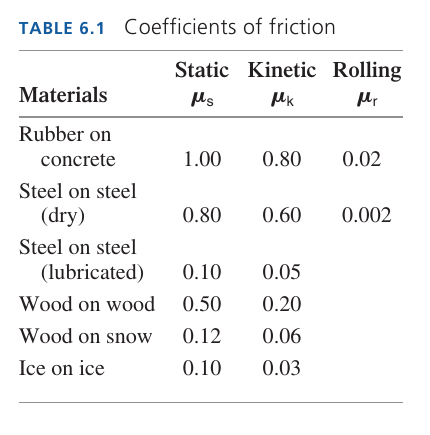
\includegraphics[width=0.5\textwidth]{mu-table.png}}
}

  \frame{\frametitle{\textbf{Sample questions}}
    \Large

    A block slides down a track elevated at angle $\theta$ with $\mu_k$ known; what is its acceleration?
  }

\frame{\frametitle{\textbf{Sample questions}}
    \Large
  A block with mass $m$ on a track is connected by a rope to a hanging weight of mass $M$. The coefficients of friction are $\mu_s$ and $\mu_k$. What is the acceleration of both objects?

  }

  \end{document}


  \frame{\frametitle{\textbf{Sample questions}}
    \Large

    Two masses of 20 and 40 kg hang from a massless pulley on either side. How do they move?
  }

  \frame{\frametitle{\textbf{Sample questions}}
    \Large

    Two masses of $m_1$ and $m_2$ kg hang from a massless pulley on either side. How do they move?
  }


\frame{\frametitle{\textbf{Summary}}
    \Large
    \BI
  \item{Forces: anything that pushes or pulls}
  \item{Forces cause accelerations: $\sum \vec F = m \vec a$}
    \BI
  \item{If $\sum \vec F = 0$, $\vec a = 0$: motion at a constant velocity}
  \EI
  \item{Forces come in pairs: if A pushes on B, B pushes back on A}
  \item{It's the vector sum $\sum \vec F$ that matters}
  \item{Draw force diagrams to keep all of this straight}
    \EI
  }



  \end{document}

